\documentclass[12pt,a4paper]{article}

% ── Packages ────────────────────────────────────────────────────────────────────
\usepackage[utf8]{inputenc}
\usepackage[T1]{fontenc}
\usepackage[english]{babel}
\usepackage{geometry}
\geometry{margin=2.5cm}

\usepackage{graphicx}
\usepackage{float}
\usepackage{subcaption}
\usepackage{booktabs}
\usepackage{tabularx}
\usepackage{longtable}
\usepackage{array}
\usepackage{multirow}
\usepackage{xcolor}
\usepackage{listings}
\usepackage{hyperref}
\usepackage{parskip}
\usepackage{enumitem}
\usepackage{fancyhdr}
\usepackage{titlesec}
\usepackage{caption}
\usepackage{amsmath}
\usepackage{tikz}
\usetikzlibrary{positioning, arrows.meta, shapes.geometric}

% ── Colors ──────────────────────────────────────────────────────────────────────
\definecolor{mongogreen}{RGB}{0,104,74}
\definecolor{codebg}{RGB}{245,245,245}
\definecolor{commentgreen}{RGB}{50,130,80}
\definecolor{keywordblue}{RGB}{30,80,180}
\definecolor{stringorange}{RGB}{180,80,20}
\definecolor{primarycolor}{RGB}{63,185,80}
\definecolor{secondarycolor}{RGB}{88,166,255}

% ── Listings (code) ─────────────────────────────────────────────────────────────
\lstset{
  basicstyle=\ttfamily\footnotesize,
  backgroundcolor=\color{codebg},
  keywordstyle=\color{keywordblue}\bfseries,
  stringstyle=\color{stringorange},
  commentstyle=\color{commentgreen}\itshape,
  numberstyle=\tiny\color{gray},
  numbers=left,
  numbersep=8pt,
  frame=single,
  rulecolor=\color{gray!40},
  breaklines=true,
  showstringspaces=false,
  captionpos=b,
  tabsize=4,
}

% ── Headers / Footers ───────────────────────────────────────────────────────────
\pagestyle{fancy}
\fancyhf{}
\rhead{\small CENG465 --- Spring 2026}
\lhead{\small Single-Leader Replication: MongoDB Fleet Management Demo}
\cfoot{\thepage}
\renewcommand{\headrulewidth}{0.4pt}

% ── Section formatting ──────────────────────────────────────────────────────────
\titleformat{\section}{\large\bfseries\color{mongogreen}}{{\thesection.}}{0.5em}{}[\titlerule]
\titleformat{\subsection}{\normalsize\bfseries}{{\thesubsection}}{0.5em}{}
\titleformat{\subsubsection}{\normalsize\itshape}{{\thesubsubsection}}{0.5em}{}

% ── Hyperref ────────────────────────────────────────────────────────────────────
\hypersetup{
  colorlinks=true,
  linkcolor=mongogreen,
  urlcolor=mongogreen,
  citecolor=mongogreen,
}

% ── Custom commands ─────────────────────────────────────────────────────────────
\newcommand{\code}[1]{\texttt{\small #1}}
\newcommand{\primary}{\textcolor{primarycolor}{\textbf{PRIMARY}}}
\newcommand{\secondary}{\textcolor{secondarycolor}{\textbf{SECONDARY}}}
\newcommand{\wmajority}{\code{w=majority}}
\newcommand{\wone}{\code{w=1}}

% ── Placeholder figure command ──────────────────────────────────────────────────
% Usage: \placeholder{width}{height}{Caption text}{label}
\newcommand{\placeholder}[4]{%
  \begin{figure}[H]
    \centering
    \fbox{\begin{minipage}[c][#2][c]{#1}
      \centering
      \textcolor{gray}{\textit{[Screenshot: #3]}}
    \end{minipage}}
    \caption{#3}
    \label{fig:#4}
  \end{figure}%
}

% ─────────────────────────────────────────────────────────────────────────────────
\begin{document}

% ── Title page ───────────────────────────────────────────────────────────────────
\begin{titlepage}
  \centering
  \vspace*{1.5cm}

  {\Large\textbf{Middle East Technical University}\\[0.3em]
  Department of Computer Engineering}

  \vspace{1cm}
  \rule{0.8\textwidth}{1pt}\\[0.4em]
  {\LARGE\bfseries\color{mongogreen}
    Data Replication in a\\[0.2em]
    Single-Leader Environment}\\[0.3em]
  {\large MongoDB Replica Set + Python Fleet Management Demo}\\[0.2em]
  \rule{0.8\textwidth}{1pt}

  \vspace{1cm}
  {\large\textbf{CENG 465 --- Principles of Data-Intensive Systems}}\\[0.5em]
  {\large Spring 2026 Project Report}

  \vspace{1.5cm}
  \begin{tabular}{ll}
    \textbf{Group:}   & Gxx \\[0.4em]
    \textbf{Members:} & Mert Karahan \\
                      & Do\u{g}ukan Top\c{c}u \\[0.4em]
    \textbf{Date:}    & June 2026 \\
  \end{tabular}

  \vfill
  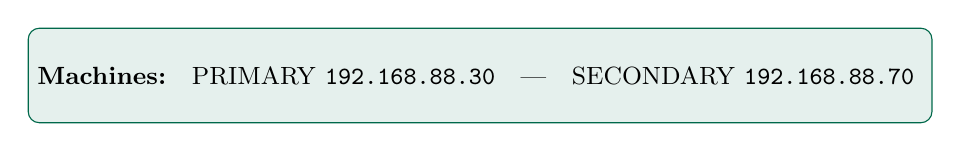
\begin{tikzpicture}
    \node[draw=mongogreen, rounded corners, fill=mongogreen!10,
          minimum width=8cm, minimum height=1.2cm, align=center, font=\small] {
      \textbf{Machines:}\quad
      PRIMARY \texttt{192.168.88.30}\quad|\quad
      SECONDARY \texttt{192.168.88.70}
    };
  \end{tikzpicture}
\end{titlepage}

% ── Table of Contents ────────────────────────────────────────────────────────────
\tableofcontents
\newpage

% ═══════════════════════════════════════════════════════════════════════════════════
\section{Introduction}
% ═══════════════════════════════════════════════════════════════════════════════════

This project implements and demonstrates \textit{single-leader replication} on two
physical macOS machines over a LAN, using MongoDB as the storage engine and a Python/Flask
control node as the client layer. The motivation is drawn directly from Chapter 5 of
\textit{Designing Data-Intensive Applications} (DDIA) by Kleppmann: replication is the
foundation of fault tolerance, read scalability, and latency reduction, but it introduces
consistency anomalies that must be explicitly handled at the application layer.

\subsection{Objectives}

\begin{enumerate}[leftmargin=2em]
  \item Deploy a two-node MongoDB replica set (\code{rs0}) on real hardware — no containers,
        no simulated latency.
  \item Implement observable write operations: every mutation records \code{leader\_write\_time},
        \code{follower\_visible\_time}, and \code{replication\_delay\_ms} in an application-level
        operation log, mirroring Raft's write-ahead log (WAL) concept.
  \item Demonstrate and measure two write concern modes: \wmajority\ (synchronous, consistency-first)
        and \wone\ (asynchronous, availability-first).
  \item Implement a fleet management domain (vehicles, drivers, depots, shipments, GPS positions,
        incidents) where each collection exhibits a different consistency requirement.
  \item Visualise three DDIA consistency guarantees — \textit{Synchronous Replication},
        \textit{Read-After-Write}, and \textit{Monotonic Reads} — as interactive DDIA-style
        timeline diagrams on the experiment dashboard.
\end{enumerate}

% ═══════════════════════════════════════════════════════════════════════════════════
\section{System Architecture}
% ═══════════════════════════════════════════════════════════════════════════════════

\subsection{Physical Topology}

The deployment uses two MacBook-class machines connected over a local Ethernet switch.
No virtualisation layer is introduced; every latency measurement reflects actual LAN
round-trip times.

\begin{table}[H]
  \centering
  \caption{Physical node inventory}
  \begin{tabular}{llll}
    \toprule
    Role           & Hostname               & IP Address       & Port  \\
    \midrule
    PRIMARY        & \code{mongo-primary.lan}   & \code{192.168.88.30} & 27017 \\
    SECONDARY      & \code{mongo-secondary.lan} & \code{192.168.88.70} & 27017 \\
    Control Node   & (macOS laptop)         & ---              & 5001 (Flask) \\
    \bottomrule
  \end{tabular}
\end{table}

\subsection{Architectural Diagram}

\begin{figure}[H]
\centering
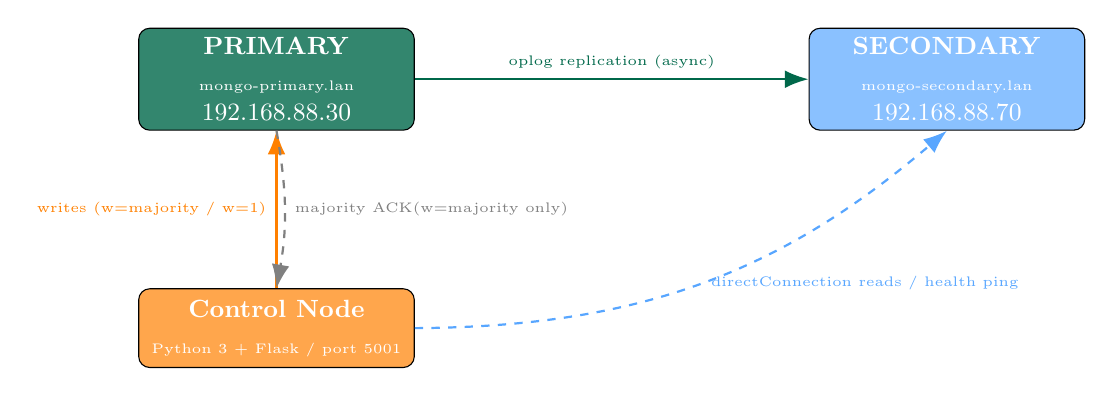
\begin{tikzpicture}[
  node distance=2cm,
  box/.style={draw, rounded corners=4pt, minimum width=3.5cm, minimum height=1cm,
              align=center, font=\small},
  arr/.style={-{Latex[length=3mm]}, thick},
]
  \node[box, fill=mongogreen!80, text=white]
    (prim) {\textbf{PRIMARY}\\[2pt]\tiny mongo-primary.lan\\192.168.88.30};

  \node[box, fill=secondarycolor!70, text=white, right=5cm of prim]
    (sec) {\textbf{SECONDARY}\\[2pt]\tiny mongo-secondary.lan\\192.168.88.70};

  \node[box, fill=orange!70, text=white, below=2cm of prim]
    (ctrl) {\textbf{Control Node}\\[2pt]\tiny Python 3 + Flask / port 5001};

  \draw[arr, color=mongogreen]
    (prim) -- node[above, font=\tiny]{oplog replication (async)} (sec);
  \draw[arr, color=orange]
    (ctrl) -- node[left, font=\tiny]{writes (w=majority / w=1)} (prim);
  \draw[arr, color=secondarycolor, dashed]
    (ctrl.east) to[bend right=20]
    node[right, font=\tiny]{directConnection reads / health ping} (sec.south);
  \draw[arr, dashed, color=gray]
    (prim.south) to[bend left=10]
    node[right, font=\tiny]{majority ACK\\(w=majority only)} (ctrl.north);
\end{tikzpicture}
\caption{Physical deployment topology. Arrows show the direction of data flow.
         Dashed arrows are conditional or health-check paths.}
\label{fig:topology}
\end{figure}

\subsection{Replica Set Configuration}

\subsubsection{Non-Voting Secondary}

A two-node replica set with equal voting rights (\code{votes=1} each) has a critical
failure mode: when the secondary goes offline, majority is lost and the primary
transitions to \textit{read-only} state — even \wone\ writes are rejected because there
is no writable primary. To avoid this, the secondary is configured as a non-voting,
zero-priority member:

\begin{lstlisting}[language={}, caption={Replica set reconfiguration at MongoDB shell}]
cfg = rs.conf()
cfg.members[1].priority = 0
cfg.members[1].votes    = 0
rs.reconfig(cfg)
\end{lstlisting}

With this configuration the primary always remains writable regardless of secondary
availability. The trade-off is that automatic failover is disabled: if the primary dies,
no election occurs. This is acceptable for a two-node demo environment.

\subsubsection{Application-Level Write Guard for \wmajority}

Because MongoDB's built-in \wmajority\ already requires the secondary to acknowledge,
it will block indefinitely when the secondary is unreachable. To give fast, deterministic
feedback, the application checks secondary reachability \textit{before} issuing the
primary mutation:

\begin{lstlisting}[language=Python, caption={Pre-write secondary reachability guard (operations.py)}]
def _require_secondary_for_majority():
    if _is_async_write():        # w=1 bypasses this guard
        return
    try:
        db.get_secondary().command("ping")
    except PyMongoError as exc:
        _set_secondary_health(False, _now(), error=exc)
        raise RuntimeError(
            "w=majority requires secondary to be reachable; "
            "write rejected before primary mutation"
        )
\end{lstlisting}

\subsection{Background Threads}

Two daemon threads run for the lifetime of the Flask process:

\begin{description}[leftmargin=2em]
  \item[\texttt{replication-log-reconciler}] Fires every \code{RECONCILE\_INTERVAL\_MS=1000ms}.
    Scans \code{operation\_logs} for \code{pending\_follower} entries and checks whether the
    secondary's document version has caught up. Closes matching log entries as
    \code{visible\_on\_follower} with a measured \code{replication\_delay\_ms}.
  \item[\texttt{secondary-healthcheck}] Fires every \code{HEALTHCHECK\_INTERVAL\_MS=1000ms}.
    Pings the secondary; on recovery, calls \code{drain\_pending\_logs()} and
    \code{sweep\_synced\_items\_from\_secondary()} to batch-close any entries that
    accumulated during an outage.
\end{description}

% ═══════════════════════════════════════════════════════════════════════════════════
\section{Schema Design}
% ═══════════════════════════════════════════════════════════════════════════════════

\subsection{Document Template}

All six fleet collections share the same envelope schema. The domain-specific content
lives in the nested \code{value} object, which varies per collection.

\begin{lstlisting}[language={}, caption={Common document schema (all fleet collections)}]
{
  _id,                // MongoDB ObjectId — primary key
  key,                // domain identifier: "VHC-001", "INC-TRK-1234..."
  value,              // nested domain object (see Table 2)
  version,            // integer, starts at 1, +1 on every write
  leader_term,        // monotonically increasing leader epoch
  last_log_index,     // foreign key into operation_logs
  last_operation_id,  // UUID — uniquely identifies the last mutation
  last_updated,       // UTC timestamp of last write
  deleted,            // boolean — soft-delete flag (no physical removal)
  created_by          // client_id string
}
\end{lstlisting}

\subsection{Why \texttt{version} Is Central}

The \code{version} field is the primary reconciliation key. When the background reconciler
runs, it reads the secondary's \code{version} for a document and compares it to the
\code{version\_after} stored in the pending log entry. If
$\text{secondary.version} \geq \text{version\_after}$, replication is confirmed and
\code{replication\_delay\_ms} is computed as:

\[
  \text{replication\_delay\_ms} = (\text{follower\_visible\_time} - \text{leader\_write\_time}) \times 1000
\]

A secondary \code{log\_index} comparison is used as a fallback when the version check
alone is ambiguous (e.g.\ after concurrent updates to the same document).

% ═══════════════════════════════════════════════════════════════════════════════════
\section{Collection Purposes and Consistency Models}
% ═══════════════════════════════════════════════════════════════════════════════════

The six fleet collections are deliberately chosen to exhibit different write frequencies
and consistency requirements, allowing all three DDIA consistency models to be
demonstrated with realistic data.

\begin{table}[H]
  \centering
  \caption{Fleet collections, consistency models, and read routing}
  \small
  \begin{tabularx}{\textwidth}{lllXl}
    \toprule
    Collection   & Write Freq. & Consistency Model  & Rationale                                              & Read From \\
    \midrule
    \code{vehicles}  & Very low    & Eventual Consistency   & Vehicle registry rarely changes; stale type/plate is acceptable.    & SECONDARY \\
    \code{drivers}   & Low         & Eventual Consistency   & Driver assignments change at depot level; minutes of lag OK.        & SECONDARY \\
    \code{depots}    & Very low    & Eventual Consistency   & Near-static reference data (city, coordinates).                      & SECONDARY \\
    \code{shipments} & Medium      & Monotonic Reads        & Status must not go backwards: \texttt{delivered}$\nrightarrow$\texttt{pending}. & SECONDARY \\
    \code{positions} & Very high   & Eventual Consistency   & GPS pings; fleet heatmap tolerates seconds of lag.                  & SECONDARY \\
    \code{incidents} & Medium      & Read-After-Write       & Safety-critical: dispatcher must see own report instantly.          & PRIMARY   \\
    \bottomrule
  \end{tabularx}
\end{table}

\subsection{Index Design}

Each collection has compound indexes tailored to its dominant access pattern, avoiding
collection scans on the secondary:

\begin{lstlisting}[language=Python, caption={Index definitions (db.py)}]
# shipments — active list ordered by recency
pdb["shipments"].create_index(
    [("value.status", ASCENDING), ("last_updated", DESCENDING)],
    name="shipments_status_updated",
)
# incidents — safety dashboard: open + severity
pdb["incidents"].create_index(
    [("value.resolved", ASCENDING), ("value.severity", ASCENDING)],
    name="incidents_resolved_severity",
)
# positions — latest GPS ping for vehicle X
pdb["positions"].create_index(
    [("value.vehicle_id", ASCENDING), ("last_updated", DESCENDING)],
    name="positions_vehicle_updated",
)
\end{lstlisting}

% ═══════════════════════════════════════════════════════════════════════════════════
\section{Logging Mechanism}
% ═══════════════════════════════════════════════════════════════════════════════════

\subsection{Operation Log Schema}

Every insert, update, and delete produces exactly one entry in \code{operation\_logs}:

\begin{lstlisting}[language={}, caption={operation\_logs document schema}]
{
  operation_id,           // UUID — unique per operation
  leader_term,            // Raft-style leader epoch
  log_index,              // global monotonic counter (Raft log index)
  operation_type,         // "insert" | "update" | "delete"
  target_collection,      // "vehicles" | "shipments" | ... | "items"
  target_id,              // ObjectId of the affected document
  leader_write_time,      // UTC — when PRIMARY committed
  follower_visible_time,  // UTC — when SECONDARY showed version_after (null initially)
  replication_delay_ms,   // float — (follower_visible_time - leader_write_time) * 1000
  version_before,         // integer — document version before the mutation
  version_after,          // integer — document version after the mutation
  client_id,              // who initiated the write
  write_concern,          // "majority" | 1
  status                  // "pending_follower" | "visible_on_follower" | "timeout"
}
\end{lstlisting}

\subsection{Log Lifecycle}

\begin{figure}[H]
\centering
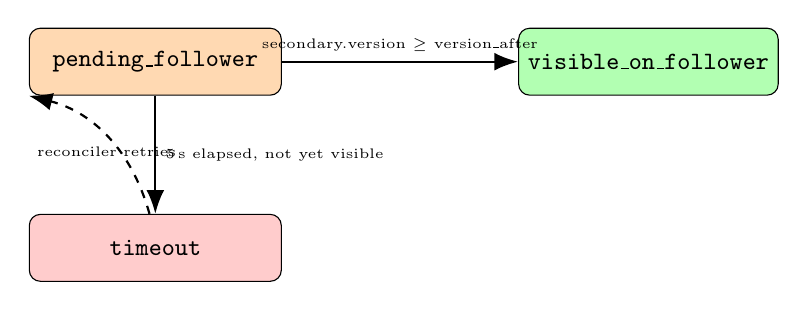
\begin{tikzpicture}[
  state/.style={draw, rounded corners=4pt, minimum width=3.2cm, minimum height=0.85cm,
                align=center, font=\small},
  arr/.style={-{Latex[length=3mm]}, thick},
]
  \node[state, fill=orange!30]   (pending)  {\code{pending\_follower}};
  \node[state, fill=green!30,   right=3cm of pending]
                                 (visible)  {\code{visible\_on\_follower}};
  \node[state, fill=red!20,     below=1.5cm of pending]
                                 (timeout)  {\code{timeout}};

  \draw[arr] (pending) -- node[above, font=\tiny]{secondary.version $\geq$ version\_after} (visible);
  \draw[arr] (pending) -- node[right, font=\tiny]{5\,s elapsed, not yet visible} (timeout);
  \draw[arr, dashed] (timeout) to[bend right=30]
    node[below, font=\tiny]{reconciler retries} (pending.south west);
\end{tikzpicture}
\caption{Log entry lifecycle. The reconciler moves entries from \code{pending\_follower}
         to \code{visible\_on\_follower} once the secondary confirms the version.}
\label{fig:lifecycle}
\end{figure}

\subsection{Completion Paths}

\paragraph{Synchronous path (\wmajority).}
After the primary commits and MongoDB returns, the application immediately polls the
secondary for up to \code{POLL\_TIMEOUT\_MS = 5\,000\,ms} at \code{10\,ms} intervals.
When the secondary's version matches, \code{follower\_visible\_time} is stamped and
\code{replication\_delay\_ms} is computed inline. The log is closed before the HTTP
response is returned to the client.

\paragraph{Asynchronous path (\wone).}
The write returns immediately; the log remains \code{pending\_follower}. Two background
threads close it later:

\begin{itemize}
  \item The \textbf{reconciler} scans pending entries every second and checks secondary
        version equality.
  \item The \textbf{health-check loop}, on detecting a secondary recovery event, drains
        all accumulated pending entries by calling \code{drain\_pending\_logs()} and
        \code{sweep\_synced\_items\_from\_secondary()}.
\end{itemize}

\subsection{Role of \texttt{target\_collection}}

A single \code{operation\_logs} collection serves all six fleet collections plus the
legacy \code{items} collection. The reconciler uses \code{target\_collection} to know
\textit{which} collection to query for the matching document. Without this field, the
reconciler would query the wrong collection and pending logs would never close —
causing \code{pending\_count} to grow unboundedly.

\begin{lstlisting}[language=Python, caption={Reconciler routing via target\_collection (operations.py)}]
for log in logs:
    collection = log.get("target_collection", "items")  # routing key
    if _secondary_has_state(
        target_id, version_after, log_index, operation_id,
        collection=collection                            # correct collection!
    ):
        _mark_log_visible(log["_id"], leader_write_time)
\end{lstlisting}

% ═══════════════════════════════════════════════════════════════════════════════════
\section{Testing Replication and Consistency Behavior}
% ═══════════════════════════════════════════════════════════════════════════════════

\subsection{Automated Test Suite (\texttt{test\_replication.py})}

Running \code{python test\_replication.py} on the control node executes seven tests
against the live replica set. All fleet collections are dropped and recreated at the
start to ensure a clean state.

\begin{table}[H]
  \centering
  \caption{Automated test suite summary}
  \small
  \begin{tabularx}{\textwidth}{llX}
    \toprule
    Test & Consistency Focus & What it proves \\
    \midrule
    1. Basic CRUD        & ---                & Insert→Update→Delete: secondary version matches primary at each step \\
    2. Fleet Static      & Eventual           & vehicles/drivers/depots replicate to the correct collection; \code{target\_collection} routing works \\
    3. Shipment Monotonic & Monotonic Reads   & Shipment status \texttt{pending}$\to$\texttt{in\_transit}$\to$\texttt{delivered} — secondary version list is always non-decreasing \\
    4. Position Burst    & Eventual           & 10 GPS inserts; avg/max \code{replication\_delay\_ms} measured; all 10 eventually appear on secondary \\
    5. Incident RAW      & Read-After-Write   & Zero-wait PRIMARY read immediately after \wone\ incident insert always returns the new document \\
    6. Async w=1 Window  & Eventual           & \wone\ GPS burst: some reads are stale right after write; after 2\,s all documents are present on secondary \\
    7. Op-Log Routing    & ---                & \code{operation\_logs.target\_collection} correctly records the collection name for every insert \\
    \bottomrule
  \end{tabularx}
\end{table}

\subsubsection{Example: Monotonic Reads Assertion (Test 3)}

\begin{lstlisting}[language=Python, caption={Monotonicity check in test\_shipment\_monotonic\_reads()}]
secondary_versions = []
for new_status in ["pending", "in_transit", "in_transit", "delivered"]:
    update_item(shp_id, {"status": new_status, ...}, collection="shipments")
    doc = db.get_secondary()["shipments"].find_one({"_id": shp_id})
    secondary_versions.append(doc["version"])

monotonic = all(
    secondary_versions[i] <= secondary_versions[i + 1]
    for i in range(len(secondary_versions) - 1)
)
# Expected: [2, 3, 4, 5] -> PASS
# Should never be: [2, 3, 2, 5] -> FAIL (impossible with single oplog stream)
\end{lstlisting}

%% TODO: Replace the placeholder below with a screenshot of test_replication.py terminal output
\placeholder{0.85\textwidth}{5cm}{Terminal output of test\_replication.py showing all 7 tests PASS}{test-output}

\subsection{Interactive Experiment Dashboard}

The Flask dashboard at \url{http://localhost:5001/experiments} provides four runnable
experiments, each producing a DDIA-style communication timeline diagram. Time flows
left-to-right; horizontal bands on a node's lane indicate processing time; diagonal
arrows show inter-node messages.

% ─────────────────────────────────────────────────────────────────────────────────
\subsubsection{Experiment 1 — Synchronous Replication (\wmajority)}
% ─────────────────────────────────────────────────────────────────────────────────

\paragraph{Protocol.}
The client writes a GPS position to PRIMARY with \wmajority. MongoDB does not return
\code{ok} until SECONDARY has replayed the oplog entry and acknowledged. The application
measures the total round-trip and decomposes it into sub-timings using a one-way network
latency estimate from a pre-experiment ping sequence.

\paragraph{Timeline shape.}
\[
  \underbrace{0 \to \text{net}_p}_{\text{request}} \quad
  \underbrace{\text{net}_p \to d - \text{net}_p}_{\text{primary processing + oplog}} \quad
  \underbrace{d - \text{net}_p \to d}_{\text{ok to client}}
\]
where $d$ is the measured total write duration and $\text{net}_p$ is the estimated
one-way latency to PRIMARY.

\paragraph{Key observation.}
The \primary\ lane shows a wide horizontal processing band: it is blocked waiting for
SECONDARY's ACK before releasing \code{ok}. This band directly visualises the
\textit{synchronous replication penalty}.

%% TODO: Replace with screenshot of Synchronous Replication experiment timeline
\placeholder{0.95\textwidth}{7cm}{DDIA-style timeline: Synchronous Replication (w=majority) --- wide processing band on PRIMARY visible}{exp-sync}

% ─────────────────────────────────────────────────────────────────────────────────
\subsubsection{Experiment 2 — Eventual Consistency (\wone\ + Artificial Delay)}
% ─────────────────────────────────────────────────────────────────────────────────

\paragraph{Protocol.}
A baseline document (\code{v1}) is established on both nodes. A 2-second
\code{secondaryDelaySecs} is set via \code{replSetReconfig}. A \wone\ update to
\code{v2} is issued; \code{ok} returns immediately. Seven secondary reads follow at
200\,ms, 500\,ms, 1\,000\,ms, 1\,500\,ms, 2\,000\,ms, 2\,500\,ms, and 3\,000\,ms after
the write. The delay is reset to zero before the function returns.

\paragraph{Key observation.}
Reads within the 2-second delay window return \code{v1} (stale). Once the oplog
propagates, reads switch to \code{v2} (fresh). This visualises the
\textit{eventual consistency window} — the period during which the system is inconsistent.

%% TODO: Replace with screenshot of Eventual Consistency experiment timeline
\placeholder{0.95\textwidth}{7cm}{DDIA-style timeline: Eventual Consistency --- stale reads (red arrows) followed by fresh reads (green)}{exp-eventual}

% ─────────────────────────────────────────────────────────────────────────────────
\subsubsection{Experiment 3 — Read-After-Write (DDIA Figure~5-3)}
% ─────────────────────────────────────────────────────────────────────────────────

\paragraph{The anomaly.}
A user writes to PRIMARY with \wone\ (fire-and-forget). If their next read is
load-balanced to SECONDARY, the oplog may not have arrived yet — the user's own write is
invisible. This is the \textit{Read-After-Write} anomaly.

\paragraph{The fix.}
Route reads to PRIMARY for the session that performed the write. PRIMARY always has the
latest committed data.

\paragraph{Protocol.}
A critical incident is inserted with \wone. Immediately:
\begin{enumerate}
  \item PRIMARY is queried → always returns the new document (\textit{RAW guaranteed}).
  \item SECONDARY is queried → may return \code{null} if oplog has not arrived (\textit{anomaly visible}).
\end{enumerate}
The actual replication delay is measured by polling the secondary after the anomaly is
detected, giving a precise \code{replication\_delay\_ms} for the timeline.

%% TODO: Replace with screenshot of Read-After-Write experiment timeline
\placeholder{0.95\textwidth}{7cm}{DDIA-style timeline: Read-After-Write --- PRIMARY read (green, always fresh), SECONDARY read (red when stale)}{exp-raw}

\paragraph{Timeline structure (DDIA Fig.~5-3 equivalent).}
Three actors are shown: \textbf{Client / Dashboard}, \primary, \secondary.
\begin{itemize}
  \item Write arrow: \textbf{Client} $\to$ \primary\ (\wone, returns immediately).
  \item Oplog arrow: \primary\ $\dashrightarrow$ \secondary\ (async, measured delay).
  \item Read 1 (correct path): \textbf{Client} $\to$ \primary\ $\to$ \textbf{Client}
        (\textcolor{green!60!black}{\textbf{$\checkmark$ fresh}}).
  \item Read 2 (wrong path): \textbf{Client} $\to$ \secondary\ $\to$ \textbf{Client}
        (\textcolor{red}{\textbf{$\lightning$ stale}} if oplog not yet applied).
\end{itemize}

% ─────────────────────────────────────────────────────────────────────────────────
\subsubsection{Experiment 4 — Monotonic Reads (DDIA Figure~5-4)}
% ─────────────────────────────────────────────────────────────────────────────────

\paragraph{The guarantee.}
If a client always reads from the \textit{same} replica, it will never observe a version
lower than one it has already seen. The classic violation occurs when a load balancer
routes consecutive reads to different replicas at different replication lag levels.

\paragraph{Protocol.}
A shipment is inserted with \wone. The actual replication delay to SECONDARY is measured
via polling. Three sequential reads are then issued to the \textit{same} SECONDARY.
The version sequence is checked for monotonicity.

\paragraph{Key observation.}
On a fast LAN, the secondary catches up in $\approx 5\,\text{ms}$, so all three reads
return \code{v1} (\code{[1, 1, 1]}). This is still monotonic and demonstrates the
guarantee. On a slower link or with \code{secondaryDelaySecs}, earlier reads may return
\code{v0} (not yet synced), but never \code{v1} then \code{v0}.

\begin{lstlisting}[language=Python, caption={Monotonicity assertion in experiment runner}]
versions = [r["version"] for r in reads]
monotonic = all(versions[i] <= versions[i + 1] for i in range(len(versions) - 1))
# [1, 1, 1] -> monotonic = True  (MONOTONIC HOLDS)
# [1, 1, 0] -> monotonic = False (MONOTONIC VIOLATED -- should not happen)
\end{lstlisting}

%% TODO: Replace with screenshot of Monotonic Reads experiment timeline
\placeholder{0.95\textwidth}{7cm}{DDIA-style timeline: Monotonic Reads --- three sequential SECONDARY reads, versions non-decreasing}{exp-monotonic}

\subsection{Manual Secondary Failure Test}

The following sequence was executed manually to validate the write guard and catch-up
detection:

\begin{enumerate}
  \item Secondary machine is taken offline (network unplugged).
  \item \wmajority\ write attempted → immediately rejected with
        \code{RuntimeError: w=majority requires secondary to be reachable}.
        No primary mutation occurs; no \code{operation\_logs} entry is created.
  \item Write concern switched to \wone.
  \item Insert succeeds on PRIMARY; \code{sec.ver = ---}; log status = \code{pending\_follower}.
  \item Secondary machine brought back online.
  \item MongoDB oplog replay begins; within $\sim$1\,s the reconciler detects
        \code{secondary.version = version\_after}; log status transitions to
        \code{visible\_on\_follower} with \code{replication\_delay\_ms} recorded.
\end{enumerate}

%% TODO: Insert 3-panel figure: (a) rejected write, (b) w=1 pending, (c) recovery synced
\begin{figure}[H]
  \centering
  \begin{subfigure}[b]{0.32\textwidth}
    \fbox{\begin{minipage}[c][4cm][c]{\textwidth}
      \centering\small\textcolor{gray}{\textit{[Screenshot: w=majority write rejected — secondary offline]}}
    \end{minipage}}
    \caption{\wmajority\ rejected}
    \label{fig:fail-majority}
  \end{subfigure}
  \hfill
  \begin{subfigure}[b]{0.32\textwidth}
    \fbox{\begin{minipage}[c][4cm][c]{\textwidth}
      \centering\small\textcolor{gray}{\textit{[Screenshot: w=1 write accepted, log pending\_follower]}}
    \end{minipage}}
    \caption{\wone\ accepted, pending}
    \label{fig:pending}
  \end{subfigure}
  \hfill
  \begin{subfigure}[b]{0.32\textwidth}
    \fbox{\begin{minipage}[c][4cm][c]{\textwidth}
      \centering\small\textcolor{gray}{\textit{[Screenshot: secondary back, log visible\_on\_follower]}}
    \end{minipage}}
    \caption{Recovery \& catch-up}
    \label{fig:recovery}
  \end{subfigure}
  \caption{Secondary failure and recovery sequence. Left: write guard rejects before primary
           mutation. Centre: \wone\ write accepted with \code{pending\_follower} status.
           Right: oplog replay completes and reconciler closes the log entry.}
  \label{fig:failure-sequence}
\end{figure}

% ═══════════════════════════════════════════════════════════════════════════════════
\section{Performance Measurements}
% ═══════════════════════════════════════════════════════════════════════════════════

%% TODO: Fill in actual values from experiment runs and benchmark.py

\subsection{Replication Latency}

One-way network latency between the control node and each MongoDB instance was measured
before each experiment run using MongoDB \code{ping} RTT divided by two
(\code{\_measure\_net\_one\_way}). Representative values observed during testing:

\begin{table}[H]
  \centering
  \caption{Measured network and replication latencies (LAN)}
  \begin{tabular}{lrrl}
    \toprule
    Metric                                & Min   & Avg   & Notes \\
    \midrule
    One-way latency to PRIMARY (net\_p)   & \textit{X.X} ms & \textit{X.X} ms & ping RTT / 2 \\
    One-way latency to SECONDARY (net\_s) & \textit{X.X} ms & \textit{X.X} ms & ping RTT / 2 \\
    \wmajority\ write total               & \textit{X.X} ms & \textit{X.X} ms & includes oplog ACK \\
    \wone\ write total                    & \textit{X.X} ms & \textit{X.X} ms & primary only \\
    Async oplog propagation delay         & \textit{X.X} ms & \textit{X.X} ms & polled from secondary \\
    \bottomrule
  \end{tabular}
\end{table}

%% TODO: Add bar chart or table from benchmark.py results

\subsection{Write Concern Overhead}

The synchronous replication overhead (\wmajority\ minus \wone\ write duration) directly
measures the cost of the ACK round-trip to SECONDARY. On our LAN this was approximately:

\[
  \text{overhead} \approx 2 \times \text{net}_s + \text{secondary\_apply\_time}
\]

%% TODO: Insert figure from benchmark results

% ═══════════════════════════════════════════════════════════════════════════════════
\section{Discussion}
% ═══════════════════════════════════════════════════════════════════════════════════

\subsection{Durability--Availability Trade-off}

The experiment confirms the fundamental tension described in DDIA Chapter 5:

\begin{itemize}
  \item \wmajority\ provides strong durability: a committed write is guaranteed to
        survive a primary crash because at least one other member (the secondary) has
        acknowledged it. The cost is latency ($\approx$ one full oplog round-trip) and
        unavailability when the secondary is unreachable.
  \item \wone\ provides high availability: writes always succeed on the primary
        regardless of secondary state. The cost is potential data loss if the primary
        crashes before the oplog propagates, and temporary read inconsistency
        (stale secondary reads).
\end{itemize}

\subsection{Consistency Anomalies on a Fast LAN}

Our LAN produces round-trip times of $< 1\,\text{ms}$, which means the secondary
typically syncs within $5\,\text{ms}$ of a \wone\ write. This makes stale reads
difficult to observe without artificial delay (\code{secondaryDelaySecs}). The
Eventual Consistency experiment explicitly introduces a 2-second delay to make the
anomaly visible. Real-world deployments across data centres or WAN links would observe
these anomalies naturally.

\subsection{Single Oplog Stream Prevents Backwards Reads}

MongoDB's oplog is a strictly ordered, append-only log. A secondary applies oplog entries
in \textit{log index order}, so the version field on any document can only increase on
the secondary. This is why the Monotonic Reads guarantee holds naturally when reading
from a single fixed secondary: you may see stale versions, but you will never see a
version go backwards.

\subsection{Limitations and Future Work}

\begin{itemize}
  \item \textbf{Two-node, non-voting secondary:} automatic failover is disabled.
        A three-node replica set with an arbiter would enable re-election.
  \item \textbf{No partitioned secondary for Consistent Prefix Reads:} DDIA Figure 5-5
        requires at least two secondaries at different replication lags to demonstrate
        out-of-order read anomalies. Our single-secondary setup cannot reproduce this.
  \item \textbf{Application-level log vs.\ oplog:} our \code{operation\_logs} duplicates
        some information already in MongoDB's native oplog. A production system would
        integrate with the oplog via change streams instead.
\end{itemize}

% ═══════════════════════════════════════════════════════════════════════════════════
\section{Conclusion}
% ═══════════════════════════════════════════════════════════════════════════════════

This project implemented a complete single-leader replication system on real hardware
and demonstrated three consistency models from DDIA Chapter 5:

\begin{enumerate}
  \item \textbf{Synchronous Replication (\wmajority):} PRIMARY waits for SECONDARY ACK.
        Every write is durable; latency penalty equals one oplog round-trip.
  \item \textbf{Read-After-Write:} routing reads to PRIMARY for the writing session
        guarantees the writer always sees their own write, regardless of secondary lag.
  \item \textbf{Monotonic Reads:} pinning all reads from a session to the same replica
        ensures version numbers never decrease, even when that replica lags behind the primary.
\end{enumerate}

The application-level operation log (\code{operation\_logs}) provides full observability:
every write is tracked from \code{leader\_write\_time} through \code{follower\_visible\_time},
making replication delay a first-class, measured metric rather than an invisible side effect.

The DDIA-style timeline visualisations on the experiment dashboard translate these abstract
consistency properties into concrete, observable message sequences — directly linking
implementation to the theoretical model.

% ═══════════════════════════════════════════════════════════════════════════════════
\appendix
\section{File Structure}
% ═══════════════════════════════════════════════════════════════════════════════════

\begin{lstlisting}[language={}, caption={Repository layout}]
ceng465_project/
  control_node/
    app.py               -- Flask application (routes, API endpoints)
    config.py            -- Connection strings, timeouts, collection names
    db.py                -- MongoDB client singletons + index creation
    operations.py        -- Write/read layer: CRUD, fleet helpers, reconciler
    experiment_runner.py -- 4 consistency experiments + DDIA event builder
    test_replication.py  -- Automated test suite (7 tests)
    benchmark.py         -- Write latency benchmarks
    templates/
      index.html         -- Fleet management dashboard
      experiments.html   -- DDIA timeline experiment runner
  presentation/
    main.tex             -- LaTeX Beamer slides
  report/
    main.tex             -- This report
    figures/             -- Screenshots and diagrams
\end{lstlisting}

\section{Write Concern API Reference}
\label{app:api}

\begin{table}[H]
  \centering
  \caption{Key configuration constants (config.py)}
  \begin{tabular}{lrl}
    \toprule
    Constant                     & Value   & Purpose \\
    \midrule
    \code{POLL\_INTERVAL\_MS}    & 10 ms   & Reconciler secondary poll cadence \\
    \code{POLL\_TIMEOUT\_MS}     & 5\,000 ms & Maximum wait for synchronous confirmation \\
    \code{WRITE\_TIMEOUT\_MS}    & 5\,000 ms & MongoDB wire-level write timeout \\
    \code{RECONCILE\_INTERVAL\_MS} & 1\,000 ms & Background reconciler loop cadence \\
    \code{HEALTHCHECK\_INTERVAL\_MS} & 1\,000 ms & Secondary health check cadence \\
    \code{SERVER\_SELECTION\_TIMEOUT\_MS} & 800 ms & MongoDB driver timeout \\
    \bottomrule
  \end{tabular}
\end{table}

\end{document}
